\section{Introduction}
\label{introduction}



%%%%%%%%%%%%%%%%%%%%%%%%%%%%%%%%%%%%%%%%%%%%%%%%%%%%%%%%%%%%%%%%%%%%%%
%%%%%%%% Figure 1
%%%%%%%%%%%%%%%%%%%%%%%%%%%%%%%%%%%%%%%%%%%%%%%%%%%%%%%%%%%%%%%%%%%%%%

\begin{figure}[t]
\begin{center}
% \fbox{\rule{0pt}{2in} \rule{0.9\linewidth}{0pt}}
   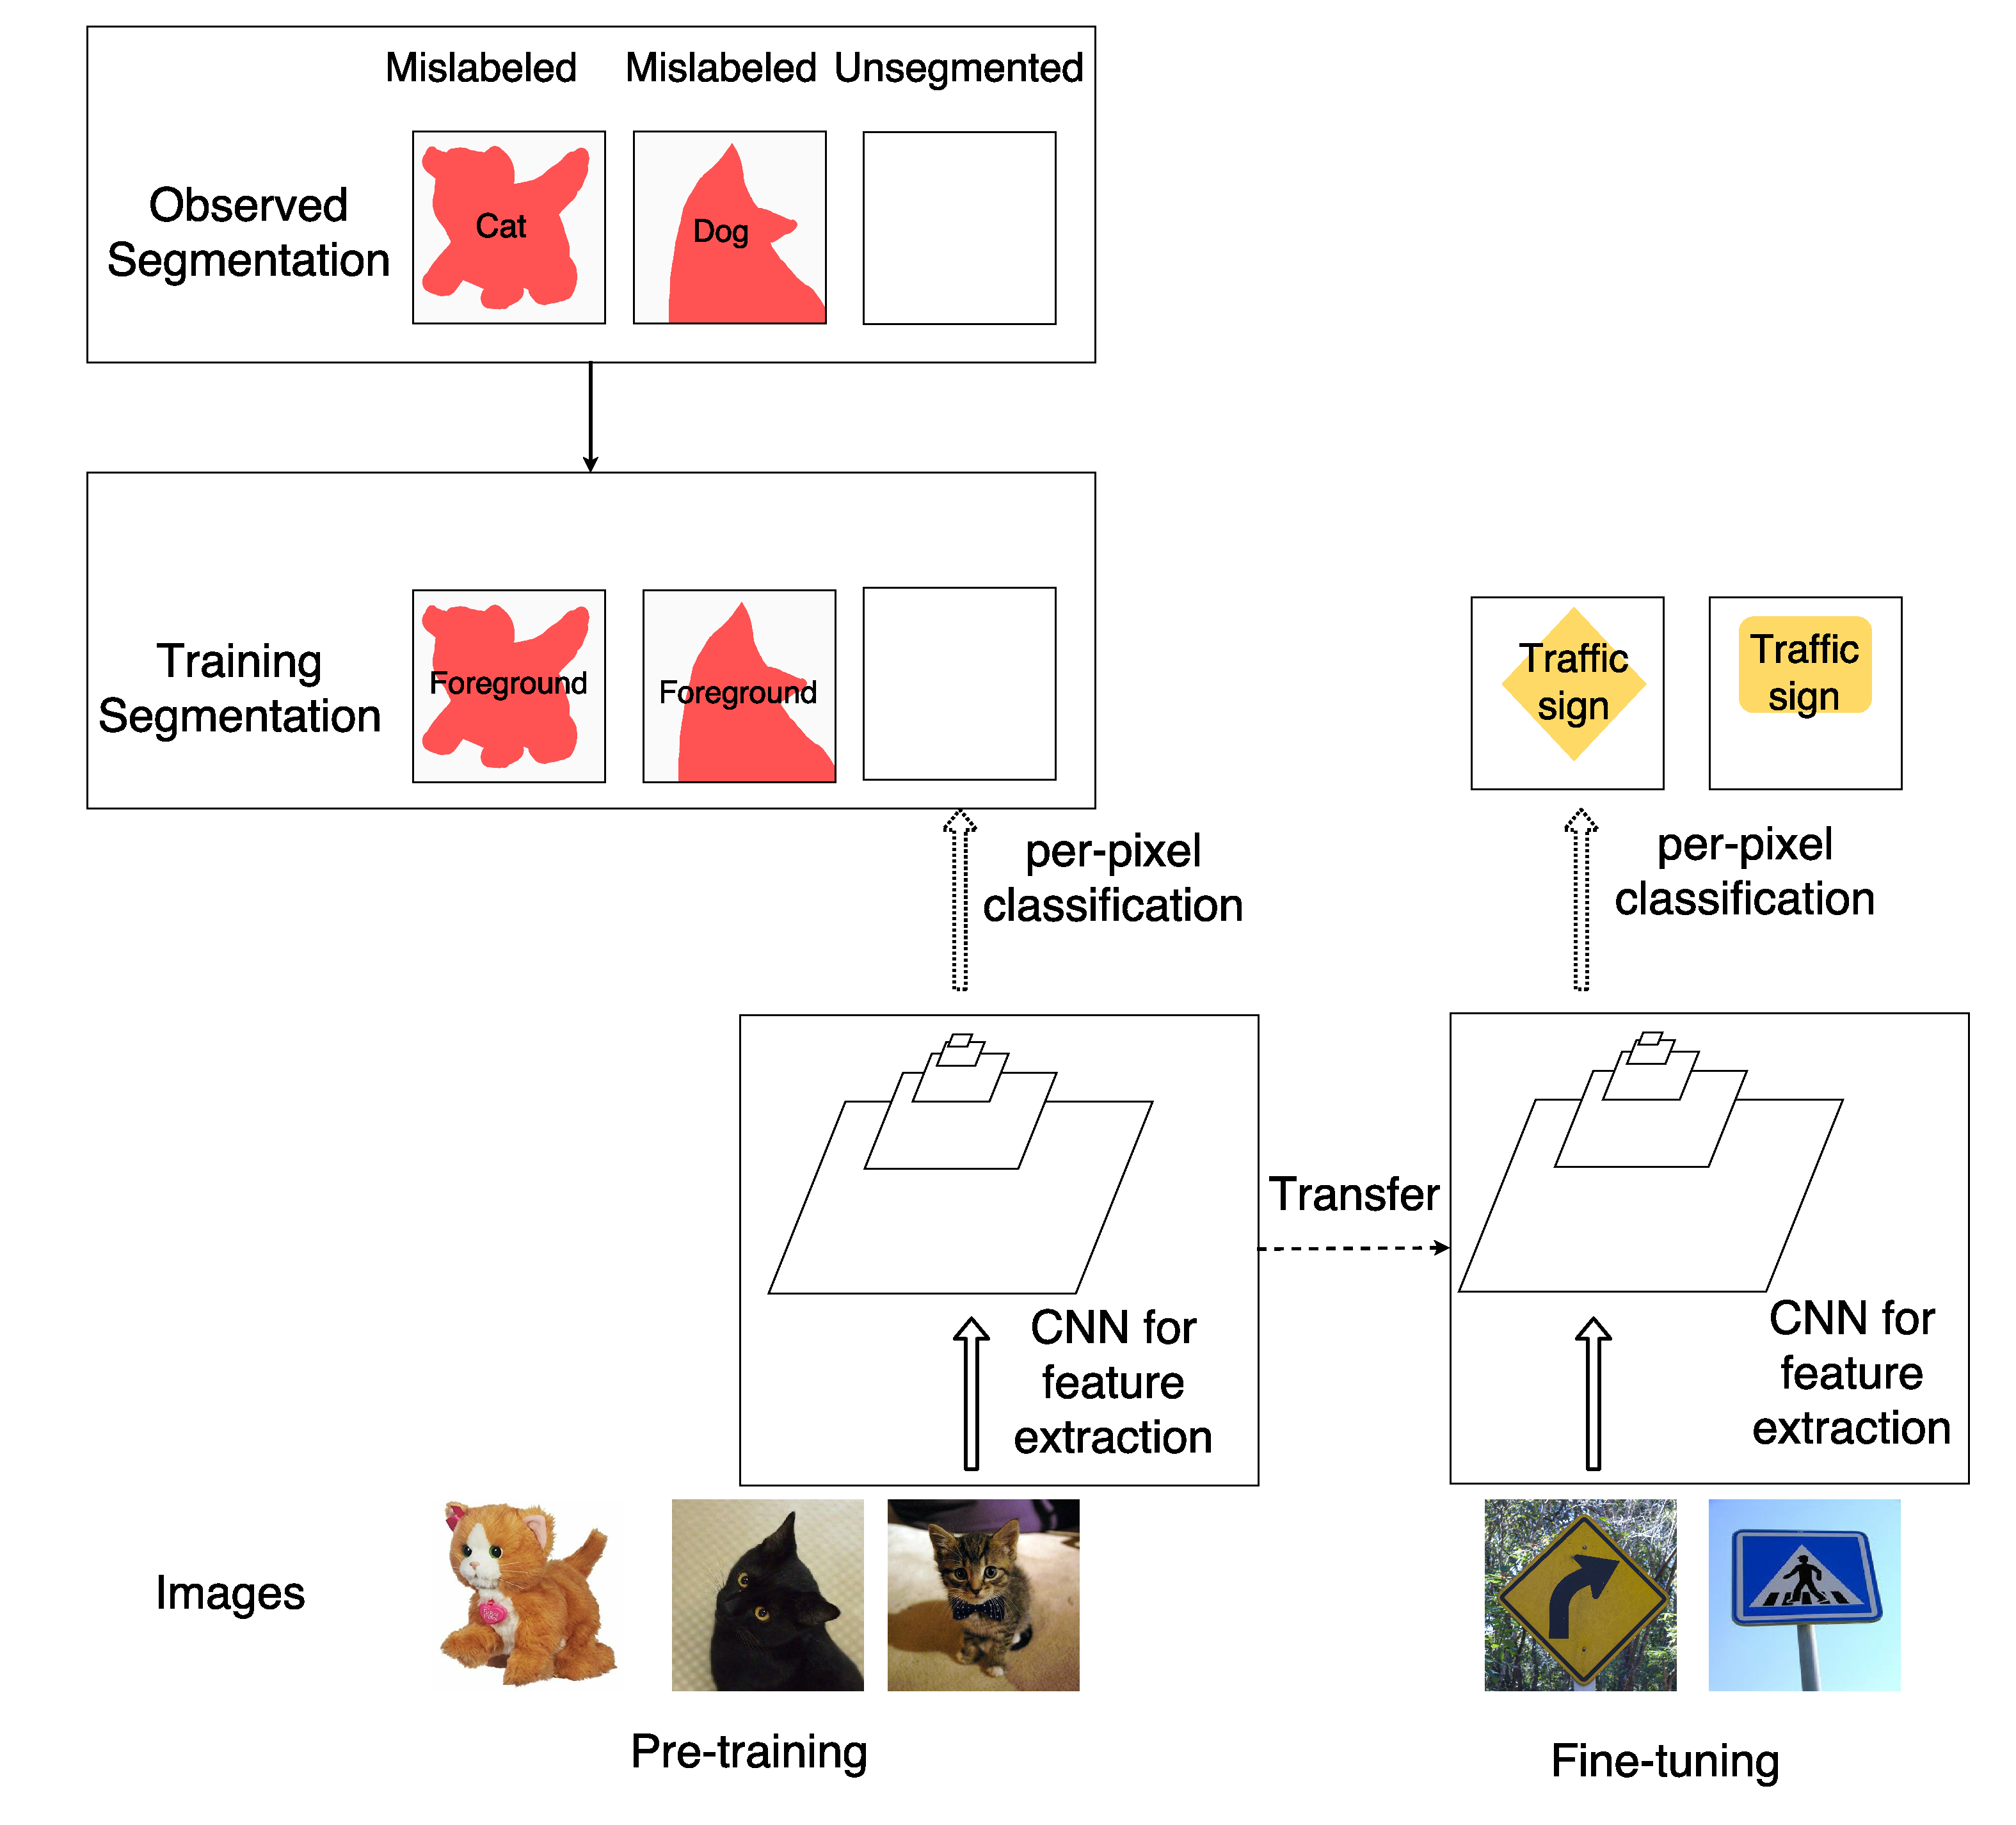
\includegraphics[width=1.1\linewidth]{img/figure1}
\end{center}
   \caption{
   Transferring the segmentation models pre-trained in the presence of segmentation noises such as inexhaustive segmentation, misclassification of objects and false segmentation.
   The convolution neural network (CNN) for feature extraction is transferred and fine-tuned with a small set of clean annotations in the domain of interest.
   }
\label{fig:long}
\label{fig:onecol}
\end{figure}


%%%%%%%%%%%%%%%%%%%%%%%%%%%%%%%%%%%%%%%%%%%%%%%%%%%%%%%%%%%%%%%%%%%%%%
%%%%%%%% TEXT Why transfer learning?
%%%%%%%%%%%%%%%%%%%%%%%%%%%%%%%%%%%%%%%%%%%%%%%%%%%%%%%%%%%%%%%%%%%%%%

% \noindent \textit{Why transfer learning? \\
% Segmentation model benefits from transfer learning.
% \begin{itemize}
%   \item Success of CNN benefits from large-scale data whereas segmentation datasets are small
%   \item Collecting segmentation in one domain on a large scale can be difficult.
%   \item One can transfer pre-trained CNN model to train with limited training samples access.
% \end{itemize}
% }

The state-or-the-art convolution neural nets benefits from transferring weights from convolutional neural network (CNN) models trained with a subset of images from ImageNet, referred to as the \textit{ImageNet models}.\cite{long2015fully,chen2016deeplab,he2017mask}
These ImageNet CNN models\cite{krizhevsky2012imagenet,simonyan2014very,szegedy2015going,he2016deep} trained for object recognition task benefit from the availability of a large-scale supervised dataset, the ILSRVC dataset\cite{russakovsky2015imagenet} which contains around 1.2 million labeled images.
In contrast to object recognition tasks, it is difficult to collect a dataset for semantic segmentation on that large scale.
This difficulty is natural because it costs much more efforts for people to segment than to classify an image.
Therefore, scales of semantic segmentation datasets are normally much smaller than object recognition dataset.
For instance, one of the largest segmentation datasets, Microsoft COCO2014\cite{lin2014microsoft}, contains 123,287 images for 80 object categories, smaller than the ILSRVC dataset by a factor of 10 approximately.
% the Pascal VOC2012 challenge\cite{everingham2015pascal} provides a segmentation dataset with only 9,993 segmented images for 20 object categories;
% The PASCAL-context Dataset\cite{mottaghi2014role} enriches the PASCAL VOC dataset by segmenting all 11,530 training images for 540 categories;
Therefore, semantic segmentation models are often trained with constraints of limited numbers of available training images.
A commonly used method for improving segmentation performance in the limitation of lacking training samples is to transfer weights from the pre-trained ImageNet models.\cite{long2015fully,chen2016deeplab}


%%%%%%%%%%%%%%%%%%%%%%%%%%%%%%%%%%%%%%%%%%%%%%%%%%%%%%%%%%%%%%%%%%%%%%
%%%%%%%% TEXT Why pre-training with segmentation?
%%%%%%%%%%%%%%%%%%%%%%%%%%%%%%%%%%%%%%%%%%%%%%%%%%%%%%%%%%%%%%%%%%%%%%

% \noindent \textit{Why pre-training with segmentation? \\
% ImageNet models have limitations.
% \begin{itemize}
%   \item Disimilarity in domain of interest for training images
%   \item Architecture limitation of ImageNet models. (3D ConvNet)
% \end{itemize}
% }

However, there can be limitations for these ImageNet models to significantly improve performance for a segmentation model.
Firstly, the ImageNet models were trained with relatively low-resolution natural images.
In some domains of interest, training images can be non-natural, for example, aerial images, images from bird's eye view, and medical images;
In other domains, mages may have different lighting conditions from the ImageNet images such as photos taken in dark warehouses;
Images to be segmented may also have higher resolution than the ImageNet ones.
To train a segmentation model in these domains, it can be beneficial to fine-tune the ImageNet model using a similar dataset in the domain of interest if there exists one.
Secondly, the ImageNet models cannot be applied directly to RGB-D images or 3D images like CT scans and MRI scans in 3D.
Lastly, segmentation models may have different design thinkings from classification models due to the inherent differences between the two tasks.
For example, features' translation invariance and reduced resolution for object recognition CNN models can reduce localization accuracy for segmentation.\cite{zheng2015conditional,chen2016deeplab}
The challenges in adapting ImageNet models for segmentation tasks can result in different architectures for segmentation models\cite{zheng2015conditional}.
% Even adapted segmentation models\cite{long2015fully,chen2016deeplab,he2017mask} have components not from the original ImageNet models.
Therefore, a model pre-trained with segmentation datasets in a similar domain can be valuable to achieve good segmentation performance with a small training set.

% \footnote{The KITTI Vision Benchmark Suite http://www.cvlibs.net/datasets/kitti/}

%%%%%%%% ? Deeplab https://arxiv.org/pdf/1606.00915.pdf
%%%%%%%% In particular we consider three challenges in the application of DCNNs to semantic image segmentation: (1) reduced feature resolution, (2) existence of objects at multiple scales, and (3) reduced localization accuracy due to DCNN invariance.
%%%%%%%% ? CRFasRNN http://www.robots.ox.ac.uk/~szheng/papers/CRFasRNN.pdf
%%%%%%%% Firstly, traditionalCNNs have convolutional filters with large receptivefields and hence produce coarse outputs when restructured to produce pixel-level labels [37]
%%%%%%%% Secondly, CNNs lack smoothness constraints that encourage label agreement between similar pixels, and spatial and appearance consistency of the labelling output


%%%%%%%%%%%%%%%%%%%%%%%%%%%%%%%%%%%%%%%%%%%%%%%%%%%%%%%%%%%%%%%%%%%%%%
%%%%%%%% TEXT Why labels are noisy?
%%%%%%%%%%%%%%%%%%%%%%%%%%%%%%%%%%%%%%%%%%%%%%%%%%%%%%%%%%%%%%%%%%%%%%

% \noindent
% \textit{Why labels are noisy?
% \begin{itemize}
%   \item Crowd-sourcing data is noisy by nature.
%   \item ``gold standard'' itself can be ambiguous.
%   \item There exists free available noisy segmentation datasets
% \end{itemize}
% }

The pre-training segmentation datasets may, however, contain label noises, and the existence of segmentation noises should not magnificently affect the transferability of pre-trained weights.
The use of the crowd-sourcing platform like Mechanical Turk is common nowadays to collect datasets on a large scale.
However, it is natural for crowd-sourcing workers to make mistakes as a result of lack of expertize, inherent ambiguity of tasks or unconscious bias.
Enormous efforts are required, according to \cite{lin2014microsoft,everingham2015pascal}, to ensure the correctness of segmentations.
A slight decrease in the percentage of segmentation errors, such as from 1\% to 0\%, may require extraordinary extra efforts due to the difficulty of identifying errors.
If not requiring ``gold standard'' segmentations, the efforts saved for correctness can be made for segmenting more images so that the result segmentations can be larger in numbers though traded with the existence of label noises.
% Trade-offs need to be made between the impact of by label noise and the gain of a larger dataset.
In some domains, for example, medical imaging, the ``gold standard'' itself can be ambiguous and cause disagreements among experts.
\footnote{TODO M: But that's OK or not?  This is what probabilities solve...}
Besides, freely available labels may exist for particular tasks, as alternatives to manual annotations.
But these labels often contain structural noises depending on the way they were created.
For example, one can use digital maps, like OpenStreetMap, to segment aerial images.
These segmentations constructed from maps would suffer from the incomplete annotation as well as registration problems.\cite{mnih2012learning}
% Besides, Pl@ntNet\footnote{https://identify.plantnet-project.org/}, a crowdsourcing platform, provide millions of images of plants and corresponding labels which may or may not be correct.
Ideally, the use of these noisy datasets for pre-training should not affect the result weights transferring to another dataset.
If negative influences of label noises on weights transferability were remarkable, methods of compensating the noises then become relevant.


%%%%%%%%%%%%%%%%%%%%%%%%%%%%%%%%%%%%%%%%%%%%%%%%%%%%%%%%%%%%%%%%%%%%%%
%%%%%%%% TEXT What types of noises exist and motivate them?
%%%%%%%%%%%%%%%%%%%%%%%%%%%%%%%%%%%%%%%%%%%%%%%%%%%%%%%%%%%%%%%%%%%%%%

% \noindent \textit{What types of noises exist and motivate them?
% \begin{itemize}
%   \item Inexaustive segmentation
%   \item Misclassification
%   \item False segmentations
% \end{itemize}
% }

% \paragraph{Segmentation noises}

Noises of different kinds can exist in segmentation labels, for example, inexhaustive segmentation, misclassification of segments, false segmentation, over-segmenting, under-segmenting, etc.
In particular, we consider only noises happen to labels for the whole segments instead of individual pixels, assuming the outline of segments is always correct.
That leaves us three types of noises: inexhaustive segmentation, misclassification and false segmentation.
Inexhaustive segmentation, i.e., there exists objects left unsegmented, is one of the most frequent noises.
A typical situation of inexhaustive segmentation is when images contain massive amounts of objects of the same kind, e.g., a flock of sheep or a pile of products.
Misclassification of segments can be avoided to some extent by asking annotators to segment one category at a time.\cite{lin2014microsoft}
Occasional misclassified objects may nevertheless still exist because of the ambiguity of category definitions, for example, the misclassified bears and teddy bears in the Microsoft COCO dataset.
False segmentation denotes that not-of-interested objects are wrongly segmented as objects of interest.
It may occur due to unclear category definition, the lack of knowledge or simply visual bias.
We synthesized these three types of noises with a well-annotated dataset and studied their influences to the trained weights transferability separately.


%%%%%%%%%%%%%%%%%%%%%%%%%%%%%%%%%%%%%%%%%%%%%%%%%%%%%%%%%%%%%%%%%%%%%%
%%%%%%%% TEXT Why binarizing classes?
%%%%%%%%%%%%%%%%%%%%%%%%%%%%%%%%%%%%%%%%%%%%%%%%%%%%%%%%%%%%%%%%%%%%%%

% \noindent \textit{Why binarizing classes?}

Supposing misclassification had a negative influence on feature transferability, as we will show in Section \ref{subsec:robustness}, a straightforward way of correcting noisy labels is to binarize classes: positive for foreground pixels and negative for background pixels.
Jain et al.\cite{jain2017pixel} trained a fully convolutional network to generate foreground segmentations, and the trained model was demonstrated generalize well for object categories not included in the training.
Binarizing classes can be considered as converting precise but inaccurate labels to accurate but imprecise labels.
For convolutional feature pre-training, precise supervision is likely not to transfer, because transferability of features is correlated to if features are general, i.e., if they depend on particular categories.
% There are a few examples proved  the possibility of training binary object detection/segmentation:
% Ren et al.\cite{ren2015faster} trained CNN model to perform binary classification for region of interest proposals;
% He et al.\cite{he2017mask} trained binary segmentation in addition to object detection for instance-aware segmentation;

%%%%%%%%%%%%%%%%%%%%%%%%%%%%%%%%%%%%%%%%%%%%%%%%%%%%%%%%%%%%%%%%%%%%%%
%%%%%%%% TEXT Why PU learning
%%%%%%%%%%%%%%%%%%%%%%%%%%%%%%%%%%%%%%%%%%%%%%%%%%%%%%%%%%%%%%%%%%%%%%

If we consider inexhaustive segmentation only the problem becomes similar to a so-called \textit{positive and unlabelled learning} (PU learning) setup\cite{li2005learning}.
In the positive and unlabeled learning setup, the training dataset has two sets of examples: the \textit{positive (P) set}, containing only positive examples, and the \textit{unlabeled (U) set}, containing a mix of positive or negative examples.
The P set in an incompletely segmented dataset is comprised of segmented pixels while the rest of the pixels construct the U set.
The main characteristic of the U set is that there is no easy way to generate reliable negative labels out of it so that the traditional semi-supervised learning techniques are not applicable as a result of the absence of negative training samples.
The set of background pixels containing unsegmented objects can fulfill this property of U set.
Learning to segment objects in the presence of inexhaustive segmentation can be thus considered as a learning problem with only positive examples and unlabeled examples.

% \noindent
% Experiments in Section \ref{subsec:robustness} indicates that inexhaustive segmentation can have significant negative influences on feature transferability.
% Besides, including mis-segmented objects for training can aggravate the inexhaustive segmentation problem.
% For example, the existence a mis-segmented toy dog does not mean that every toy dogs are mis-segmented.
% The other unsegmented toy dogs then become a source of inexhaustive segmentation and lead to worse fine-tuning performance as we discovered in Section \ref{sec:experiments}.
% Method to compensate inexhaustive segmentation is therefore necessary to train better transferable representation.

%%%%%%%%%%%%%%%%%%%%%%%%%%%%%%%%%%%%%%%%%%%%%%%%%%%%%%%%%%%%%%%%%%%%%%
%%%%%%%% TEXT Main contributions
%%%%%%%%%%%%%%%%%%%%%%%%%%%%%%%%%%%%%%%%%%%%%%%%%%%%%%%%%%%%%%%%%%%%%%

To summary, the main topics discussed in this thesis are:
\begin{enumerate}
  \item We investigated the influence of labels noises on feature transferability for semantic segmentation.
  \item Binarizing classes for pre-training can alleviate the effect caused by the existence of misclassification of segments.
  \item We proposed a class-dependent loss for negative examples to compensate the influence of unsegmented objects of interest.
\end{enumerate}



%%%%%%%%%%%%%%%%%%%%%%%%%%%%%%%%%%%%%%%%%%%%%%%%%%%%%%%%%%%%%%%%%%%%%%
%%%%%%%% TEXT Table of contents
%%%%%%%%%%%%%%%%%%%%%%%%%%%%%%%%%%%%%%%%%%%%%%%%%%%%%%%%%%%%%%%%%%%%%%

The rest of this thesis is organized as follows:
In the next section, we summarize related works.
 % in areas of transfer learning, deep learning with noisy labels and PU learning.
In Section \ref{sec:robustness} we formulate the problem of pre-training with noisy segmentations and how to synthesize the three types segmentation noises.
We proposed a sigmoidal loss for noisy negative samples in Section \ref{sec:pulearning}.
Experiments in Section \ref{subsec:robustness} was designed to study the influences of inexhaustive segmentations, misclassification and false segmentation separately.
The proposed sigmoidal loss, together with the class-weighted loss and a modified hard bootstrapping loss, was evaluated in synthesized PU learning setups in Section \ref{subsec:pulearning}.
Discussions are included in Section \ref{sec:discussion} and conclusions are summarized in Section \ref{sec:conclusion}.
%Features learned by predicting the pixel objectness with inexaustive annotations were then validated with experiments described in Section \ref{sec:discussion}.
